\documentclass[notitlepage,letterpaper,12pt]{article} % para articulo

% Este es un comentario <- Los comentarios comienzan con % 
% todo lo que se escriba hasta el final de la linea será ignorado <- Este es otro comentario

%Lenguaje del documento
\usepackage[spanish]{babel} % silabea palabras castellanas <- Puedo poner comentarios para explicar de que va este comando en la misma línea

%Encoding
\usepackage[utf8]{inputenc} % Acepta caracteres en castellano
\usepackage[T1]{fontenc} % Encoding de salida al pdf

%Hipertexto
\usepackage[colorlinks=true,urlcolor=blue,linkcolor=blue]{hyperref} % navega por el doc: hipertexto y links

%simbolos matemáticos
\usepackage{amsmath}
\usepackage{amsfonts}
\usepackage{amssymb}

% permite insertar gráficos, imágenes y figuras, en pdf o en eps
\usepackage{graphicx} 
\usepackage{epstopdf}

% geometría del documento, encabezados y pies de páginas, márgenes
\usepackage{geometry}     
\geometry{letterpaper}       % ... o a4paper o a5paper o ... 
\usepackage{fancyhdr} % encabezados y pies de pg
\pagestyle{fancy}
\chead{\bfseries {Aquí va el Título del documento}}
\lhead{} % si se omite coloca el nombre de la seccion
\rhead{fecha del doc}
\lfoot{\it Autor  }
\cfoot{Universidad Industrial de Santander}
\rfoot{\thepage}
%margenes
\voffset = -0.25in
\textheight = 8.0in
\textwidth = 6.5in
\oddsidemargin = 0.in
\headheight = 20pt
\headwidth = 6.5in
\renewcommand{\headrulewidth}{0.5pt}
\renewcommand{\footrulewidth}{0,5pt}

\begin{document}
\title{Título del Informe}
\author{
\textbf{Nombre y Apellido Autor1\thanks{e-mail: \texttt{autor1@uis.edu.co}}}\\
\textbf{Nombre y Apellido Autor2\thanks{e-mail: \texttt{autor2@uis.edu.co}}}\\
\textit{Nombre de la institución}\\
\textit{Dirección de la institución}\\
} % Hasta aquí llega el bloque "author" (son dos autores por informe, orden alfabético)

\date{Versión $\alpha \beta$ fecha del documento}
\maketitle %Genera el título del documento
\tableofcontents %Genera la tabla de contenidos (índice)

%Resumen
\begin{abstract}
Y aquí el resumen. El resumen debe ser suficiente para que uno no se lea el documento. Toda la información importante y trascendente del documento debe estar aquí. Típicamente debe tener una extensión entre 400 a 500 palabras.
\end{abstract}

%Introducción
\section{Introducción}

Aquí debe ir la descripción del problema, su importancia, sus antecedentes. Seguidamente la justificación de este reporte, por qué se hace esta investigación, como se enmarca en los antecedentes y cuál es su importancia. Es importante, en la introducción mostrar como se enmarca los logros alcanzados en este trabajo con los antecedentes que los precedieron. Los acrónimos deben ser explicitados la primera vez que aparezcan.

Quizá la mejor recomendación es consultar el libro de Umberto de Cómo hacer una Tesis Doctoral: ECO, U. ?Como Se Hace Una Tesis: Técnicas y Procedimientos de Estudio, Investigacion y Escritura/  Col. Libertad y Cambio. Serie Práctica. \footnote{\url{http://web.usal.es/~mom/tesis_eco.pdf}}


Esta sección se finaliza con una descripción de lo que viene. Qué contienen cada una de las secciones.

%Metodología
\section{Metodología}
En esta sección se echa el cuento de cómo se montó el experimento. La metodología experimental o teórica utilizada, sus detalles y haciendo referencia a los antecedentes. Cuáles herramientas (o técnicas) se utilizaron. El por qué se utilizaron: cuáles son las ventajas y las desventajas de esas herramientas.

% Puedo usar subsecciones para destacar un serie de párrafos que forman un marco común dentro de una sección:
\subsection{Tablas}
Las Tablas deben ser lo más autocontenidas posibles. Sus títulos y  leyendas deben ser suficiente para explicar su contenido. Las tablas deben ser referidas desde el texto (ver Tabla \ref{Tabla1}). Si no se hace referencia a una tabla en particular, ésta se considera inútil para el artículo y debe ser suprimida

%Ejemplo de tabla
\begin{table}
  \centering
\begin{tabular}{l|c|r} %primera columna alineación izq (l=left), segunda alineación central (c=center) y tercera columna alineación derecha (r=right)
\hline % hline dibuja una línea horizontal
% after \\ : \hline or \cline{col1-col2} \cline{col3-col4} ... este campo se usa para multicolumna
  Evento 1 & Evento 1  & Evento 3  \\ \hline
  Justificado Izquierdo & centrado & Justificado derecho \\
   &  &  \\ \hline \hline
\hline
\end{tabular}
  \caption{Las leyendas deben explicar el contenido de las tablas} % leyenda de la tabla: comando "caption"
  \label{Tabla1} %Referencia interna: cuando quiera llamar a la tabla usare \ref{Tabla1} (ver arriba)
\end{table}

\section{El experimento}
¿ Qué se midió ? ¿ cuáles fueron las condiciones de medición ? ¿ que representan esas medidas ? ¿ cuáles son las limitaciones de la medida por las restricciones que impone la técnica y las herramientas ?

\subsection{Figuras}
Al igual que las Tablas, las Figuras deben ser lo mas autocontenidas posibles. Sus títulos y  leyendas deben ser suficiente para explicar su contenido. Las figuras deben ser referidas desde el texto (ver Figura (o Fig) \ref{Figura1}). Otra vez, si no se hace referencia a una figura en particular, ésta se considera inútil para el artículo y debe ser suprimida

\begin{figure}
\begin{center}
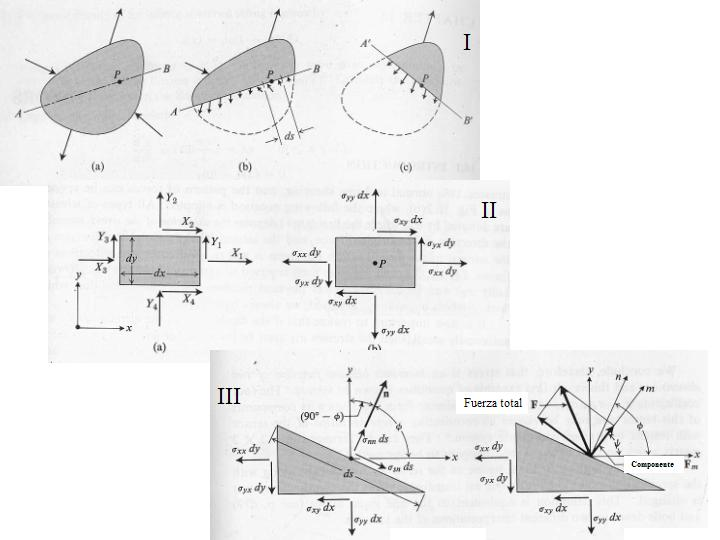
\includegraphics[width=2in]{figs/FigTensorEsfuerzos2D.jpg} % incluyo la imagen con la dirección de la misma
\caption{Esta figura incorpora una imagen}
\label{Figura1} %referencia interna de la figura 
\end{center}
\end{figure}


\section{Conclusiones y Recomendaciones}
A partir de las medidas ¿ qué se concluyó ? ¿ cuál fue el aporte de este esfuerzo ? ¿ qué se recomienda hacer ? ¿ cuáles serían los próximos pasos o acciones a tomar ?

\section{Referencias}
Aquí deben ir las referencias citadas \cite{Narasimhan1993} cuando corresponda y los url que se consideren necesarios y que hayan sido citadas en el texto del documento. Es mucho más fácil utilizar \texttt{Bibtex}, que es un mecanismo para citar referencias siguiendo los patrones internacionales. Si no se hace uso de \texttt{Bibtex} se tiene que tener cuidado de citar de la forma que lo requiera la publicación. Si no hay recomendaciones de los editores, lo mejor es apegarse a algún estilo estándar y civilizado de presentar la bibliografía Hay muchos por allí \url{http://www.researchconsultation.com/dissertation-references-thesis-citations-bibliography.asp}.

\bibliographystyle{unsrt} % estilo de las referencias 
\bibliography{BibTex/BiblioLN130519} %archivo con los datos de los artículos citados

% Forma Manual de hacer las referencias
% Se escribe todo a mano...
% Descomentar y jugar

%\begin{thebibliography}{99}
%\bibitem{Narasimhan1993}Narasimhan, M.N.L., (1993), \textit{Principles of
%Continuum Mechanics}, (John Willey, New York) p. 510.

%\bibitem{Demianski1985}Demia\'{n}ski M., (1985), \textit{Relativistic
%Astrophysics,} in International Series in Natural Philosophy, Vol 110, Edited
%by \textit{D. Ter Haar}, (Pergamon Press, Oxford).
%\end{thebibliography}


%Fin del documento
\end{document}

%Todo lo que escriba aquí será ignorado, aunque no fuera un comentario...





